%%-------------------------------------
\documentclass[12pt]{article} % Document class article only supports 10pt, 11pt, and 12pt.
\usepackage[utf8]{inputenc}
\usepackage[english]{babel}
\usepackage{cx}
\usepackage{tcolorbox}
\usepackage{geometry}
\geometry{left=3cm,right=3cm,top=2cm,bottom=2cm} %% 设置页边距:

\usepackage{indentfirst}
\usepackage{algpseudocode}




%% 行距、段距设置
%\linespread{1.2}     % 设置基本行距。
% article 文档类的默认是1,即1.2倍字号大小;
% ctexart 文档类的默认是1.3,即1.56倍字号大小。
\setlength\parskip{5pt}   % 段间距

\usepackage[
	backend=bibtex,
	style=numeric-comp,
	sorting=nyt,
	date=year,
	backref=true,
	backrefstyle=three]
	{biblatex}
\addbibresource{/Users/chenxin/Desktop/chenxin-biblatex.bib}




\newcommand{\monic}{\rightarrowtail}
\newcommand{\epic}{\twoheadrightarrow}
\newcommand{\monoepiarrow}{\rightarrowtail\hspace{-1em}\twoheadrightarrow}
\newcommand{\isoarrow}{\xrightarrow{\sim}}

% blank symbol
\newcommand{\blank}{\sqcup}

%%=============================================================================
\title{Notes on Logic, Computability \& Complexity}
\author{\textsc{Xin Chen} \qquad \href{mailto:chenxin_hello@outlook.com}{\textsf{chenxin\_hello@outlook.com}}  
	\qquad 
	$Q_{uality} = \int (\text{\Large $K$},P,t)$}
\date{latest update: \today}

%%-------------------------------------
\begin{document}


\maketitle

\begin{quotation}
	\itshape May the force of \textsf{P} and \textsf{NP} be with you. 	
\end{quotation}


\tableofcontents


\medskip

Citation testing: \cite{Aro.Bar2009}

\vspace{2em}

One of the important scientific advances in the first half of the twentieth century was that the notion of ``computation'' received a much more precise definition.


At roughly 50 years (1970s -- 2020s), 
complexity theory is still an infant science, 
and many important results are less than 30 years old.



\section{Basic concepts}


%%=============================================================================
\subsection{logarithms}


\begin{df}[Logarithms]
    Let $a,b$ be two positive real numbers, 
    and $a \neq 1$. 
    \textit{The logarithm of $b$ to the base $a$},
    denoted by {\color{purple} $\log_a b$}, 
    is the unique real number $x$ such that $a^x = b$. 
    % 
    That is, 
    \[
        \log_a b = x \quad \text{iff} \quad a^x = b.
    \]
\end{df}

The logarithm function is the inverse of the exponential function. 
% 
The logarithm function is defined for $a>0$, $a \neq 1$, and $b>0$. 
% 
The most commonly used bases are $a=2$, $a=e$, and $a=10$. 
% 
The base $a=2$ is used in computer science, 
$a=e$ is used in calculus, 
and $a=10$ is used in engineering and science. 
The base $a=10$ is called the \textit{common logarithm}, 
and is denoted by $\lg b$.

\begin{table}[ht!]
    \centering
    \caption{Commonly used bases for logarithms}
    \label{tab: logarithm}
    \vspace{1em}
    \begin{tabular}{c||c}
        \hline
        Base & Notation \\
        \hline
        $2$ & {\color{purple} $\log b$} \\
        $e$ & $\ln b$ \\
        $10$ & $\lg b$ \\
        \hline
    \end{tabular}
\end{table}

$\log_a b \quad\leadsto\quad  a^\Box = b$

$e \approx 2.718$

\begin{table}[h]
    \centering
    \renewcommand{\arraystretch}{1.3} % 行距
    \caption{Identities of logarithms}
    \vspace{1em}
    \begin{tabular}{c||l}
    \hline
    Identity & \multicolumn{1}{c}{Formula}  \\
    \hline
    
    Product & $\log_b(xy) = \log_b x + \log_b y$ \\

    Quotient & $\log_b(\frac{x}{y}) = \log_b x - \log_b y$ \\

    Power & $\log_b x^r = r \cdot \log_b x$ \\

    Root & $\log_b \sqrt[r]{x} = \frac{1}{r} \cdot \log_b x$ \\
    \hline
\end{tabular}
\end{table}






% figure
\begin{figure}[ht!]
    \centering
    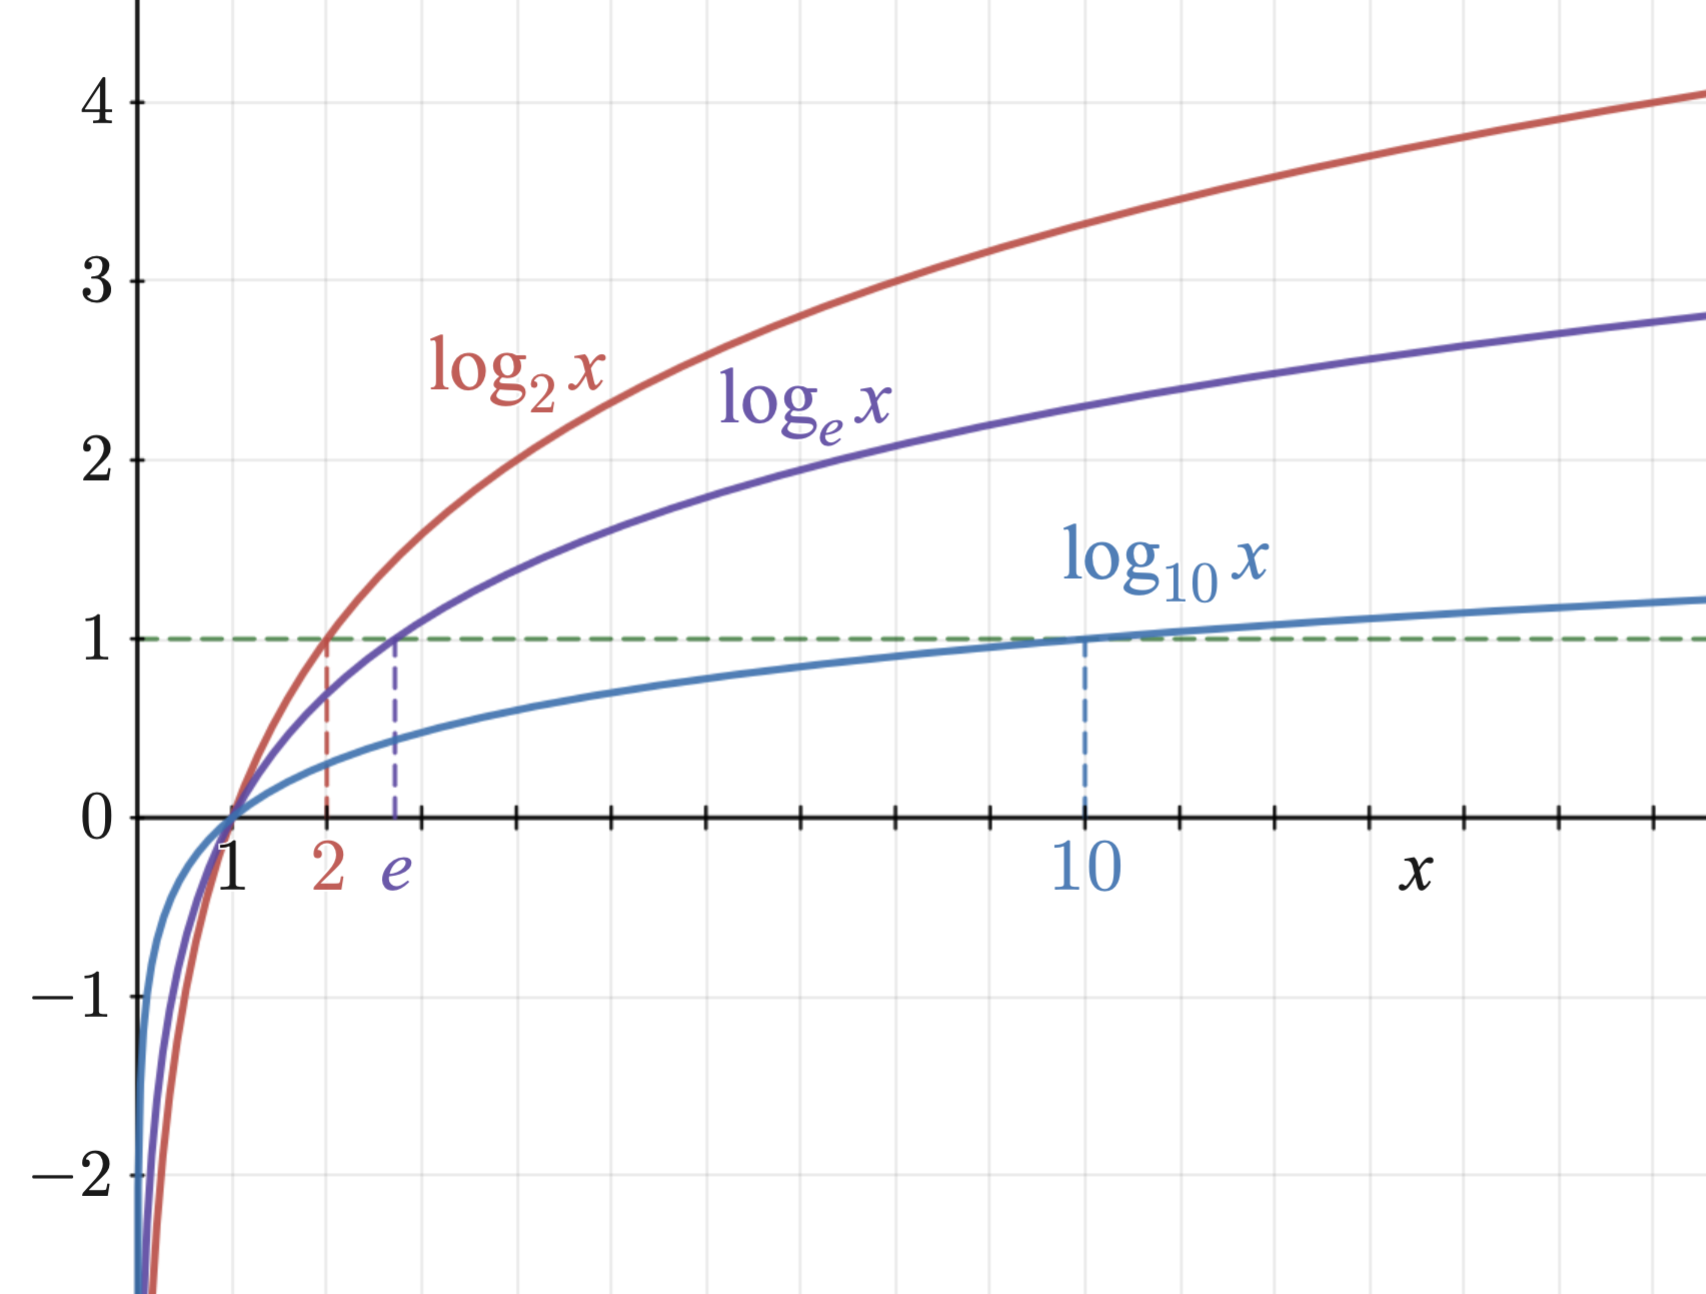
\includegraphics[width=.5\textwidth]{fig/logarithm.png}
    \caption{Plots of logarithm functions, with three commonly used bases, from \href{https://en.wikipedia.org/wiki/Logarithm}{wikipedia}}
    \label{fig: logarithm}
\end{figure}





%%=============================================================================
\subsection{Strings}

If $S$ is a \textit{finite} set, called \textit{alphabet set}, 
then a \textit{string} over $S$ is a finite ordered tuple of elements from $S$. 

We will typically consider the \textit{binary} alphabet $2 = \{0,1\}$.


$S^0 = \{\epsilon\}$

$S^* = \bigcup_{n \geq 0} S^n$ is the set of all strings over $S$.


The \textit{concatenation} of strings $x,y$ is denoted by $x^\frown y$, $x \circ y$, or simply $xy$.


$x^k$ denotes the concatenation of $k$ copies of $x$ for $k \geq 1$. 
% 
For example, 
$1^3$ is `$111$'.

The length of a string $x$ is denoted by $|x|$.


%%=============================================================================
\subsection{Representations}


we implicitly identify any function $f$ whose domain and range are not strings with the function 
\[
    g \colon \{0,1\}^* \to \{0,1\}^*
\]
that given a representation of an object $x$ as input, 
outputs the representation of $f (x)$. 


%%=============================================================================
\subsection{Big--Oh notation}



\begin{df}[Big--Oh notation]
    If $f,g$ are two functions over $\mathbb{N}$, 
    then we say that 
    \begin{enumerate}[itemsep=5pt,parsep=5pt,leftmargin=3em,topsep=5pt,label=(\arabic*)] %% or label = \alph*, \roman*
        \item 
        {\color{purple} $f = O(g)$} if there exist a constant $c$ such that $f(n) \leq c \cdot g(n)$ for every sufficient large $n$.

        \item 
        $f = \Omega(g)$ if $g = O(f)$.

        \item 
        $f = \Theta (g)$ if $f=O(g)$ and $g=O(f)$.

        \item 
        {\color{purple} $f=o(g)$} if for $\forall \kappa > 0$, 
        $f(n) \leq \kappa \cdot g(n)$ for every sufficient large $n$.

        \item 
        $f = \omega(g)$ if $g = o(f)$.
    \end{enumerate}   

    To emphasize the input parameter, 
    we often write {\color{purple} $f(n)=O(g(n))$} instead of $f= O(g)$, 
    and use similar notation for $o,\Theta,\Omega,\omega$.
\end{df}



\begin{example}
    Here are some examples of big--Oh notation:
    \begin{enumerate}[itemsep=5pt,parsep=5pt,leftmargin=3em,topsep=5pt,label=(\arabic*)] %% or label = \alph*, \roman*
        \item 
        If $f(n)=100n\log n$ and $g(n)=n^2$, 
        then $f = O(g)$.

        \item 
        If $f(n) = 100n^2 + 24n + 2\log n$ and $g(n)=n^2$, 
        then $f=O(g)$ and $g=O(f)$.
    \end{enumerate}
\end{example}




\section{Computational models}


This section introduces some of the most important computational models in the history of computer science and explains \textit{why it doesn't matter.}



Uncomputability has an intimate connection to G\"{o}del's famous Incompleteness Theorem.



%%=============================================================================
\subsection{Turing machines}


% figure
\begin{figure}[h]
    \centering
    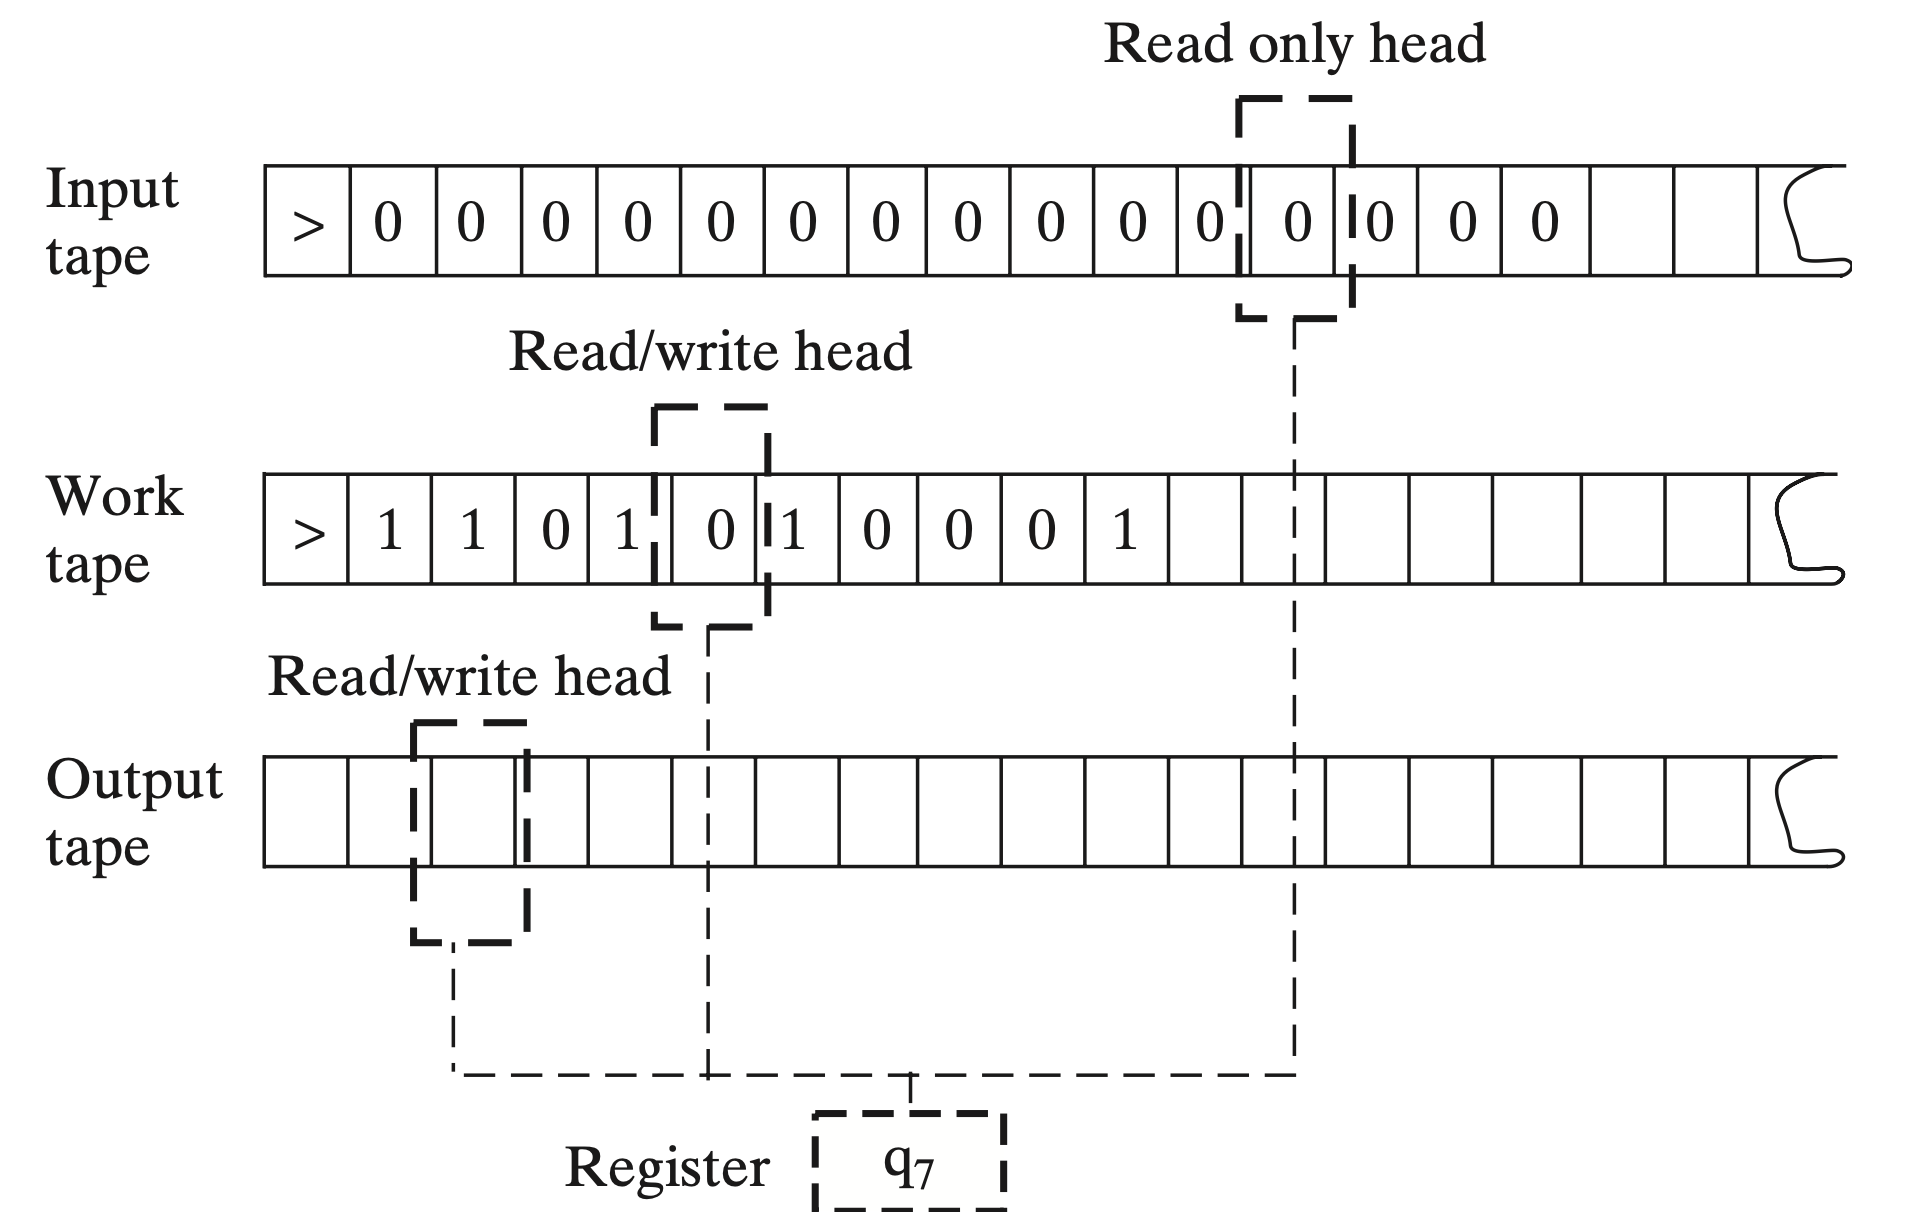
\includegraphics[width=.9\textwidth]{fig/three-tape-TM}
    \caption{A snapshot of the execution of a three--tape Turing machine M with an input tape, a work tape, and an output tape, see \cite[p.~11]{Aro.Bar2009}}
    \label{fig: three-tape-TM}
\end{figure}




A \textit{tape} is an infinite one--directional line of cells, each of which can store a symbol from a finite  set called \textit{alphabet}.
% 
Each tape is equipped with a \textit{tape head} that can potentially read or write symbols to the tape one cell at a time.



alphabet $\{0,1\} \cup \{\blank, \triangleright, \}$



state set $Q$, contains two distinguished states: 
the start state $q_{start}$ and the halting state $q_{halt}$







\begin{example}[palindrome \zh{回文}]
    A \textit{palindrome} is a string that reads the same forwards and backwards. 
    % 
    The language of palindromes over the binary alphabet is 
    \[
        PAL = \{ w \in \{0,1\}^* \mid w = w^R \}
    \]
    where $w^R$ denotes the reverse of $w$.
    % 
    For example, 
    $00100$ is a palindrome,
    and clearly $\{\epsilon,0,1\} \subseteq PAL$.
    % 
    
    A Turing machine that computes $PAL$ within less than $3|x|$ steps for any input $x$.

    Our TM $M$ will use three tapes (the input, work and output tape) and the alphabet $\{\blank,\triangleright,0,1\}$: 
    
    \vspace{1em}
    \begin{algorithmic}[1]
        \State Input $x$  (where $|x|=n$)

        \State 
        Copy $x$ to the work tape \qquad ($n$ steps)

        \State 
        Move the input--tape head the begining of $x$ \qquad ($n$ steps)

        \State 
        Move the input-tape head to the right while moving the work-tape head to the left.

        \If{at any moment the machine observes two different symbols}
            \State \textbf{reject} and output $0$
        \Else 
            \State \textbf{accept} and output $1$
        \EndIf  \qquad ($\leq n$ steps)
        \end{algorithmic}
\end{example}




%%=============================================================================
\subsection{Running Time}

Any nontrivial computational task requires at least reading the entire input, 
we count the number of basic steps as a function of the input length.



\begin{df}[Computing a function and running time]
    Given $f \colon \{0,1\}^* \to \{0,1\}^*$, 
    $T \colon \mathbb{N} \to \mathbb{N}$ and a Turing machine $M$, we say that
    % 
    \begin{enumerate}[itemsep=5pt,parsep=5pt,leftmargin=3em,topsep=5pt,label=(\arabic*)] %% or label = \alph*, \roman*
        \item $M$ \textit{computes} $f$ if for every $x \in \{0,1\}^*$, 
        whenever $M$ is initialized to the start configuration on input $x$, 
        then it halts with $f(x)$ on the output tape.

        \item 
        \textit{$M$ computes $f$ in $T(n)$--time} if its computation on every input $x$ requires at most $T(|x|)$ steps.
    \end{enumerate}
\end{df}




%%=============================================================================
\subsection{Machines as Strings and the Universal Turing Machine}

It is almost obvious that \textit{we can represent a Turing machine as a string}: 
Just write the description of the TM on paper, 
and encode this description as a sequence of zeros and ones.
% 
This string can be given as input to another Turing machine.






%%=============================================================================
\subsection{Variants of Turing machines}

\subsubsection{Turing machines with alphabet $\{0,1,\blank,\triangleright\}$}

\subsubsection{Single tape Turing machines}

\subsubsection{Bidirectional single tape Turing machines}







%%=============================================================================
\subsection{Other  computational models*}



%%-------------------------------------
\subsubsection{URM: the unlimited register machine}



\section{Uncomputability}

There exist functions that cannot be computed within any finite amount of time.









\section{The Class \textsf{P}} 

A \textit{complexity class}is a set of functions that can be computed within given resource bounds.





\begin{df}[The class \textsf{DTIME}]
    The class \textsf{DTIME}($f(n)$) is the set of all functions that can be computed by a deterministic Turing machine in $O(f(n))$ steps.
\end{df}

The \textsf{D} in the notation \textsf{DTIME} refers to ``deterministic''.



\begin{df}[The class \textsf{P}]
    The class \textsf{P} is the union of all complexity classes \textbf{DTIME}($n^c$) for all  $c$.
    % 
    In other words,
    \[
        \mathsf{P} = \bigcup_{c \geq 1} \mathsf{DTIME}(n^c).
    \]
\end{df}


P: polynomial.



\begin{example}[Graph connectivity]
    Graph connectivity problem: 
    
    input: a graph $G$ and two vertices $s,t$, 
    
    inquiry: whether there is a path from $s$ to $t$.

    Using \textit{depth--first search} (DFS), 
    we can solve this problem in $O(|V|+|E|)$ steps.
\end{example}







% /////////////////////////////////////////////////////////////////////////////
\clearpage
\printbibliography
\addcontentsline{toc}{section}{References}
\end{document}